\TUchapter{Background}
\TUsection{Introduction}
This chapter provides background and context for the concepts, modeling
frameworks, and example domains involved in this thesis. First, hybrid systems
and their newer counterpart, cyber physical systems, are addressed. Existing
modeling frameworks for hybrid systems, particularly hybrid automata, are
defined. Second, an introduction to attack graphs is provided along with a
survey of their areas of research.

Next, section 2.4 presents at length the basic attack graph model developed at the
University of Tulsa and the components thereof that do not represent a
contribution of this thesis. Finally, section 2.5 introduces the specific
domains of the two examples used throughout this thesis.
\TUsection{Cyber Physical Systems}
\TUsubsection{Hybrid Systems}
A system with both continuous (frequently physical) components and discrete (frequently digital)
components is said to be a \emph{hybrid system}, named for its characteristic blending of the
two domains. Examples of hybrid computer systems abound in industrial controls, for example,
although hybrid systems may also be fully physical (e.g., a bouncing ball that experiences continuous
behavior when rising and falling and discrete behavior when colliding with a surface).

The term hybrid system is an older one that was coined as researchers began to study the newly
pervasive reactive systems that arose as programmed control of the physical world became 
widespread ~\cite{alur1993hybrid}. For several reasons it does not suffice to describe precisely
the types of systems with which this work is concerned: a subset of hybrid
systems that incorporate a significant computer and networking component.

Nevertheless, the modeling of hybrid systems is well studied and provides a sufficient body
of relevent work from which to draw to warrant its inclusion. This chapter includes
background on a particularly relevent modeling framework for hybrid systems called the
hybrid automaton, which is used in this thesis as the standard benchmark against which to
compare hybrid modeling techniques.
\TUsubsection{Definition}
A newer, better term for the systems investigated in this thesis is \emph{cyber physical systems}
 (CPS).
Put simply, a cyber physical system is a networked hybrid system: a networked computer system that is 
tightly coupled to the physical world.
\TUsubsection{Challenges}
According to the 2008 Report of the Cyber-Physical Systems Summit, ``The principal barrier to 
developing CPS is the lack of a theory that comprehends cyber and physical resources in a 
single unified framework.''~\cite{summitreport2008}

The summit further identified as part of the necessary scientific and technological foundations of
cyber physical systems both (1) new modeling frameworks that ``explicitly address new observables'' and (2)
studies of privacy, trust, and security including ``theories of cyber-physical inter-dependence''~\cite{summitreport2008},
a major theme of this work.

Crenshaw and Beyer recently enumerated four principal challenges in cyber physical systems testing that are
equally apt for security:
their concentration in safety critical domains, their frequent integration of third-party or
otherwise unrelated systems, their dependence upon unreliable data collection, and their
pervasiveness~\cite{crenshaw2010upbot}.
% TODO Add more here.
\TUsubsection{Hybrid Automata}
\TUsubsubsection{Definition}
A valuable formalism for modeling hybrid systems in isolation and with limited composition
is the hybrid automaton of Alur, et al.~\cite{alur1993hybrid}. This section introduces the
version of the formalism described in 1996 by Henzinger~\cite{henzinger1996theory}, to which a
reader interested in more than a superficial understanding is referred. 

Formally,
a hybrid automaton $H$ is made up of a set of real-valued state variables, their first derivatives,
a set of operational modes and switches between the modes, and predicates attached to those modes and
switches describing the operation of the system in those modes and the discrete transitions between
them. One can think of a hybrid automaton as a pairing of a finite state machine whose states (called
modes) and transitions (called switches) denote the discrete-domain behavior of the hybrid system, with
a set of differential equations attached to each mode, which govern its continuous-domain behavior. Switches
may also be labeled in order to permit synchronization across composed hybrid automata.

Modes may be decorated with invariant conditions (which state whether the system is allowed to be in that mode),
flow conditions (which state how the continuous domain state variables are permitted to evolve while in that
mode), and initial conditions (which state under which, if any, conditions the automaton may begin its operation
with that mode). Switches are decorated with jump conditions, which serve as guards on the switch determining
both (1) when the switch is allowed to be taken, and (2) the discrete changes in state variables due to that
switch's activation.

A simple example of a hybrid automaton is given in Fig.~\ref{fig:thermostat}, which models a simple
heater thermostat~\cite{henzinger1996theory}. The vertices in the automaton represent 
its operating modes, and the edges represent its control
switches. In the ``Off'' mode, the temperature (given by $x$) must be greater than or equal to 18, and
its first derivative with respect to time (denoted $\dot{x}$) is $-0.1x$, which represents a cooling of
the environment. When the temperature is strictly less than 19, the switch from off to on is available (but
not mandatory until the off mode's invariant condition $x \geq 18$ ceases to be satisfied.) The switch from
on to off behaves similarly.

\begin{figure}
\centering
\begin{dot2tex}[options=-t raw --autosize]
digraph G {
    rankdir=LR;
    
    Off [texlbl="$\begin{matrix} \text{Off} \\ \
    \dot{x} = -0.1x \\ \
    x \geq 18 \\ \
    \end{matrix}$"];
    
    On [texlbl="$\begin{matrix} \text{On} \\ \
    \dot{x} = 5 - 0.1x \\ \
    x \leq 22 \\ \
    \end{matrix}$"];
        
    Off -> On [label=" " texlbl="$x < 19$"];
    
    On -> Off [label=" " texlbl="$x>21$"];
}
\end{dot2tex}
\caption{Thermostat hybrid automaton}
\label{fig:thermostat}
\end{figure}

The hybrid automaton model is sufficiently rich to capture many hybrid systems. 
\TUsubsubsection{Shortcomings}
There are some problems with the hybrid automaton model. A hybrid automaton is not guaranteed to
have a valid execution, and computing whether it does or not is non-trivial~\cite{lygeros1999existence}.
Model checking has been developed for only some subclasses of 
automata~\cite{henzinger1997hytech}~\cite{frehse2005phaver}, and many desirable
properties of them are undecidable~\cite{henzinger1998s}.

However, there are even more nagging problems when considering hybrid automata or their variants
for the study of cyber physical systems. One of the hallmarks of cyber physical systems is a
distributed and highly networked nature. While they provide a
natural model for the discrete-continuous boundary, hybrid automata have only a rudimentary
notion of communication, no clear means for specifying message passing, and when used in large
topologies have significant scaling problems, both computationally and cognitively.
\TUsubsubsection{Alternatives}
Some attempts have been made to solve the problem of the hybrid automaton's unsatisfactory
capability for modeling networks and communication. Particularly, the designation of shared
actions and shared variables as ``input'' or ``output'' is a popular tactic, used in the
powerful hybrid I/O automaton~\cite{lynch1996hybrid}~\cite{lynch2001hybrid}, its descendent the
timed I/O automaton~\cite{kaynar2010theory}, and also in the PHAVer model 
checker~\cite{frehse2005phaver}.

The work of this thesis is also something of an outgrowth from an instance of this strategy in
which prototypical ``hybrid link automata'' were developed to model explicit communication channels.
An example of the cognitive scalability issues inherent with this design is given in Fig.~\ref{fig:linkmachine},
a considered ``hybrid link automaton'' prototype modeling
a link on which messages may be dropped, injected, or delayed, and on which rudimentary mutual
exclusion of messages is enforced.
This strategy may have a place in modeling some systems but falls short of the goal of 
modeling complex, interdependent networks of hybrid systems with more conventional computer networks.
\begin{figure}
\centering
\begin{dot2tex}[options=-t raw --autosize]
digraph G {
    rankdir=TD;
    idle [shape=circle, texlbl= \
    "$ \begin{matrix} \lambda : \mu : \text{Idle} \\ \
    \dot{C}_{\lambda \mu} = 0 \\ \
    C_{\lambda \mu} = 0 \end{matrix} $"];
    
    transmit [shape=circle, texlbl= \
    "$ \begin{matrix} \lambda : \mu : \text{Transmit} \\ \
    \dot{C}_{\lambda \mu} = 1 \\ \
    C_{\lambda \mu} < l \wedge w_{\lambda}=1  \end{matrix}$"];
    
    wait [shape=circle, texlbl= \
    "$\begin{matrix} \lambda : \mu : \text{Wait} \\ \
    w_{\lambda}=1 \\ \
    \end{matrix}$"];
    
    transmit -> idle [label= " " \
    texlbl="$\begin{matrix} \lambda : D : \mu \\ \
    C_{\lambda \mu} < l \\ \
    C_{\lambda \mu} := 0 \wedge w_{\lambda}:=0 \
    \end{matrix}$"];
    
    idle -> transmit [label= " ", \
    texlbl= "$\begin{matrix} S : \lambda : \mu \\ \
    w_{\lambda}=0 \\ \
    w_{\lambda}:=1 \\ \
    \end{matrix}$"];
    
    idle -> wait [label= " ", \
    texlbl= "$\begin{matrix} S : \lambda : \mu \\ \
    w_{\lambda}=1 \\ \
    \end{matrix}$"];
    
    wait -> transmit [label= " ", \
    texlbl= "$\begin{matrix} \
    w_{\lambda}=0 \\ \
    w_{\lambda}:=1 \\ \
    \end{matrix}$"];
    
    wait -> wait [label= " ", \
    texlbl= "$\begin{matrix} S : \lambda : \mu \\ \
    \end{matrix}$"];
    
    idle -> idle [label= " ", \
    texlbl="$\lambda : D : \mu$"];
    
    idle -> transmit;
    
    transmit -> idle;
    idle -> idle [label= " ", \
    texlbl="$S : \lambda : \mu$"];
    
}
\end{dot2tex}
\caption{Example hybrid link automaton}
\label{fig:linkmachine}
\end{figure}

Other alternatives may exist in the realm of hybrid systems research. Although
the hybrid automata is the gold standard for modeling hybrid systems, other
frameworks do exist such as hybrid process algebras~\cite{cuijpers2005hybrid}~\cite{bergstra2005process},
an entirely symbolic system with many of the same properties and drawbacks as
hybrid automata. Hybrid Petri nets are similar to hybrid automata in that they
pair a standard discrete model (in this case, Petri nets instead of finite state
automata) with differential equations to model the continuous side of the
system or process~\cite{champagnat1998petri}. Because Petri nets are designed to
model distributed systems, hybrid Petri nets may hold some promise, though they
are not the topic of this thesis.
\TUsection{Attack Graphs}
\TUsubsection{Introduction}
An attack graph is one of several related formalisms that utilize graph theory to
model the state space of computer systems attacks. Perhaps they are best introduced
when presented as an alternative to a similar model called an attack tree.
\TUsubsection{Attack Trees}
An attack tree is a goal-oriented tree model of an abuse of a system~\cite{schneier1999modeling}.
The root of the tree represents the attacker's goal, and the children of any given node represent
the prerequisite activities required to reach that node. For example, consider the goal of
stealing a car, which is modeled in a simple attack tree in Fig.~\ref{fig:attacktree}.

The attacker must start the car and drive away; this could be accomplished either by breaking
in and hotwiring the car, or by stealing the owner's key and using it to subsequently steal the
car. The root of the tree represents the final goal of the theft, with prerequisite goals
flowing upward from the leaf nodes.
\begin{figure}
\centering
\begin{dot2tex}[options=-t raw --autosize]
digraph G {
    rankdir=BU;
    StealCar [texlbl="Steal car" shape=rectangle];
    UseKey [texlbl="Start car with key" shape=rectangle];
	HotWire [texlbl="Hotwire car" shape=rectangle];
	StealKey [texlbl="Steal owner's key" shape=rectangle];
	OpenDoor [texlbl="Access car interior" shape=rectangle];
	CallLocksmith [texlbl="\begin{tabular}{c}Impersonate owner \\to locksmith\end{tabular}" shape=rectangle];
	BreakWindow [texlbl="\begin{tabular}{c}Break in \\through window\end{tabular}" shape=rectangle];
	UseKey -> StealCar;
	HotWire -> StealCar;
	StealKey -> UseKey;
	OpenDoor -> HotWire;
	CallLocksmith -> OpenDoor;
	BreakWindow -> OpenDoor;
}
\end{dot2tex}
\caption{Simple car theft attack tree}
\label{fig:attacktree}
\end{figure}

There are a few features of this modeling method to note. It is goal oriented, meaning that
the consequences of the attack are known, and the goal is to ennumerate and and analyze the
means by which those consequences could be reached. It is, as an attack model, agnostic to the
underlying system model which makes it difficult to generate automatically. Finally, and perhaps
most significantly, it captures the ways in which an attacker's actions interact and 
depend upon each other.

This threat-centric model is not necessarily the most useful for system stakeholders. It
requires that one work backward from the attack to the system state
necessary to realize the attack. If, instead, an analyst desires to work from a system characterization
and explore the attack space permitted by that system characterization, the attack tree framework
must be in some sense turned upside down. 
Attack graphs do exactly that.
\TUsubsection{Attack Graphs}
\TUsubsubsection{Introduction}
In contrast to attack trees, attack graphs permit a topology-aware exploratory analysis of
the state space of a system. It is a graph theoretic model in which vertices represent individual
system states, and edges represent state transitions caused by an adversary. The concept as
introduced in 1998 included notions of generalized attack patterns to be bound to state transitions;
network elements and their individual configurations; network topology (three characteristics common
to all current attack graph iterations); a notion of the attacker's capabilities, and edge weights
representing likelihood~\cite{phillips1998graph}. A similar structure called a privilege graph was
introduced in 1994~\cite{dacier1994privilege}.

Most approaches to attack graph modeling represent exploits (attack patterns) using
preconditions and postconditions~\cite{lippmann2005annotated} since this was suggested in about 2000~\cite{templeton2001requires}. Exploits are chained together by matching preconditions in a state node's
underlying system model and applying their postconditions to generate a successor state.
\TUsubsubsection{Model Types}
The modeling substrates of attack graphs can be broadly separated into two schools of
thought, separated by the philosophy that guides the representation of the underlying
network model over which network states and transitions are computer.

A specification of an underlying network model may be done with only very loose
restrictions, allowing arbitrary keywords as named qualities and topoligies of network objects.
This thesis employs this method. It is also favored in the work of George Mason 
University~\cite{ammann2002scalable}~\cite{wang2006minimum}. It has the advantage of
permitting more straightforward adaptation into the continuous domain, which is the reason
it is favored by this work. 

An alternate specification method is much more restricted, confining the modeler to
certain sets of terms that may, for example, impose explicit computer networking 
comcepts onto the model~\cite{templeton2001requires}.
This permits generation and analysis to take a
more nuanced view of a network state, including reachability analysis to determine whether a
given topology permits communication between two hosts~\cite{ingols2009modeling}. This approach
is favored in the work of MIT Lincoln Laboratory and the University of California, Davis.
\TUsubsubsection{Research Directions}
Research in attack graphs is spread throughout a variety of pathways. These include
evaluating a network's security~\cite{ammann2002scalable}, specification of formal languages
to represent attack graphs~\cite{templeton2001requires}, intrusion detection system 
integration~\cite{tidwell2001modeling}, automatic generation of security recommendations~\cite{wang2006minimum},
and reachability analysis between hosts in a single network state~\cite{ingols2009modeling}. 
For a thorough literature review up to 2005 and more detailed discussion of popular research directions, 
refer to the work of Lippmann and Ingols~\cite{lippmann2005annotated}.

Attack graph work can be considered to fall into four broad categories, referenced
occasionally throughout this work by the following names.
\begin{description}
\item[Modeling] Attack graph modeling concerns the development of the underlying representation
	and use of that representation to model systems. Terminology belongs here, as do efforts to
	automatically generate network models from real networks and exploit patterns from vulnerability
	databases.
\item[Generation] Attack graph generation is the process of building a graph out of a model by
	closing the state space over its exploits. This is where most performance work is concentrated.
	A good portion of the work that enables a representation of time to be included in attack graphs
	belongs here as well. Constraints (such as monotonicity) on the way that state transitions are 
	allowed to progres also fall under the generation category.
\item[Analysis] Analysis of attack graphs focuses on drawing conclusions about a system based upon
	the attack graph generated from its model. Work here includes integration with intrusion detection
	systems, automatic delivery of mitigation recommendations, and the identification of security
	consequences with particular states.
\item[Visualization] Visualization of attack graphs seeks to reduce or eliminate their
	known cognitive scalability issues; the goal is to deliver the results of the other three
	steps in a meaningful fashion.
\end{description}

Its goal being to introduce an architecture for modeling hybrid systems with
attack graphs, this thesis is mainly concerned with the modeling stage. However, 
some amount of work is included in the generation stage, particularly
dealing with the progression of time; consideration is also given to analysis, 
particularly on identifying failure states and
on aggregating sufficiently similar states (which also touches visualization).



%%%%%%%%%%%%%%%%%%

\TUsection{Attack Graph Generation and Modeling}
This sections presents a version of the attack graph modeling framework specific
to traditional information systems. The framework has a very permissive model that
includes notions of assets, qualities, topologies. Assets represent potentially
attackable system components; qualities assign an arbitrary string value to a named
property of an asset, and topologies bind pairs of assets together with a named
connection between them. Exploit patterns with preconditions and postconditions attached
to free variables that can be bound at generation time to assets serve to describe potential
state transitions.
\TUsubsection{Intuitive Definition}
For the purposes of this work, an attack graph is comprised of the following components.
\begin{description}
	\item[Assets] Assets are the subjects in the attack graph formalism, mainly representing
		attackable system components. For example, an asset may represent a host
        on a network, an attacker, or a critical document. Assets are specified
		with unique names, and they are decorated with \emph{qualities} and \emph{topologies}.
		Assets can also be used to model users and adversaries if it is necessary to give them
		explicit properties. A model's collection of assets is fixed at definition time and
		is not changed by state transitions.
	\item[Qualities] Qualities represent properties of an asset, such as a software package or
		version that is installed, whether it is offline, online, or in sleep mode. Qualities are
		can be considered a key/value pair, where both the key and the value are string tokens. For
		example, the \texttt{host1} asset may have the quality \texttt{power} and the value \texttt{on}.
		Together with topologies, qualities make up the network state's collection of facts.
	\item[Topologies] Topologies represent relationships between two assets. These can be physical such
		as denoting that a printer is plugged into a computer, logical such as denoting that one
		host is accessible from another on an adjacent network, or more abstract such as a particular
		trust relationship or level of access that a subject has on another. Topologies are directed and
		named with string tokens. For example, \texttt{host1} might be accessible over the network via the
		web by \texttt{host2}, so a directed topology from \texttt{host2} to \texttt{host1} called
		\texttt{network\_remote\_web} might be used. Together with qualities, topologies make up the
		network state's collection of facts.
	\item[State] A network or system state is comprised of all of the facts about the system's asset
		collection. A network model's state is fully described by the asset collection and the fact base;
		given the constant asset collection, a state is uniquely described by its fact base. The fact
		base is all the qualities and topologies that are valid for that state.
	\item[Exploit patterns] Exploit patterns are generalized templates for how the actions of the attacker
		can alter the system state by inserting and removing qualities and topologies (but not assets).
		They are written as functions that take a number of parameters corresponding to assets, mapping
		a set of preconditions (facts about the free asset parameters) to a set of postconditions:
		insert and delete actions on qualities and topologies to update the fact base and therefore
		generate a new network state.
\end{description}
\TUsubsection{Formal Definition}
\TUsubsubsection{Primitive Domains}
To further clarify the data types in use by the attack graph formalism,
this section provides a more formal definition of their domains.
The primitive domains are the most basic 
domains that describe the atomic units of
the formalism: assets, properties (qualities), values (qualities), relationships (topologies),
vulnerabilities (exploit pattern identifiers), and parameters (free asset variables in the attack
patterns), and operations (used in postconditions representing insert or delete actions).
See Fig.~\ref{fig:primitivedomains}.

\begin{figure}
\begin{align*}
    \mathcal{A} :& \text{assets} \\
    \mathcal{P} :& \text{properties (quality names)} \\
    \mathcal{V} :& \text{values (property values)} \\
    \mathcal{R} :& \text{relationships (topology names)} \\
    \mathcal{W} :& \text{vulnerabilities (exploit pattern names)} \\
    \mathcal{I} :& \text{parameters (free asset names)} \\
    \text{Op} =& \left\{\text{ins}, \text{del} \right\}
\end{align*}
\caption{Attack graph primitive domains}
\label{fig:primitivedomains}
\end{figure}

\TUsubsubsection{Compound Domains}
Compound domains comprise the fundamental concepts that are composed of combinations
of members of the primitive domains. These form the level of abstraction that it is
most convenient to discuss in the articulation of the execution model and in the
preceding intuitive definition, for instance.
\begin{description}
    \item[Qualities] Qualities bind an asset to a property to a value; therefore their
        domain is the cartesian product of those domains. The $n$ subscripts denote that
        these are bound qualities of a network state, rather than free qualities in
        exploit preconditions and postconditions:
        \begin{align*}
            \mathcal{Q}_n &: \mathcal{A} \times \mathcal{P} \times \mathcal{V}
        \end{align*}
    \item[Topologies] Topologies bind an asset to another asset through a relationship; therefore their
        domain is the cartesian product of those domains:
        \begin{align*}
            \mathcal{T}_n&: \mathcal{A} \times \mathcal{A} \times \mathcal{R}
        \end{align*}
    \item[Network states] A network state, then, is denoted by a collection of assets, and a fact base
        of qualities and topologies; the domain of a network state is the cartesian product
        of the power sets of these domains:
        \begin{align*}
            \mathcal{N}&: \mathbb{P}(\mathcal{A}) \times \mathbb{P}(\mathcal{Q}_n) \times \mathbb{P}(\mathcal{T}_n)
        \end{align*}
    \item[Exploit patterns] Exploit patterns, taken from the domain $\mathcal{E}$ 
		depend upon free versions of qualities and topologies,
		which are parameterized by members of $\mathcal{I}$ rather than $\mathcal{A}$, which are used in
		preconditions and, when combined with an operator, postconditions:
        \begin{align*}
			\mathcal{Q}_e&: \mathcal{I} \times \mathcal{P} \times \mathcal{V} \\
			\mathcal{T}_e&: \mathcal{I} \times \mathcal{I} \times \mathcal{R} \\
			\text{Preconditions } \mathcal{P}rc_e &: \mathbb{P}(\mathcal{Q}_e) \times \mathbb{P}(\mathcal{T}_e) \\
			\text{Postconditions } \mathcal{P}oc_e&: \mathbb{P}((Op,\mathcal{Q}_e)) \times \mathbb{P}((Op,\mathcal{T}_e)) \\
			\mathcal{E}&: \mathcal{W} \times \vec{\mathcal{I}} \times  \mathcal{P}rc \times \mathcal{P}oc
        \end{align*}
    \item[Attacks] An exploit pattern whose parameters have been bound to assets is referred to as an
		attack. It takes a similar appearance:
		\begin{align*}
			\text{Preconditions } \mathcal{P}rc_n &: \mathbb{P}(\mathcal{Q}_n) \times \mathbb{P}(\mathcal{T}_n) \\
			\text{Postconditions } \mathcal{P}oc_n&: \mathbb{P}((Op,\mathcal{Q}_n)) \times \mathbb{P}((Op,\mathcal{T}_n)) \\
			\mathcal{X}&: \mathcal{W} \times \vec{\mathcal{I}} \times  \mathcal{P}rc \times \mathcal{P}oc
        \end{align*}
\end{description}

\TUsubsection{Network Model Specification}
The attack graph execution model expanded upon by this thesis does 
not use this formal notation to represent system elements, instead favoring a 
more user friendly specification language. This section describes that 
specification language and the generation process. % Todo: name it? :)
A network model specification consists of a list of assets and an initial fact base 
(list of qualities and topologies). It begins with the phrase \texttt{network model}, followed
by the~\texttt{=} symbol. 

The first component of the specification itself is an asset list.
The asset list is a semicolon separated list of the names of network
assets preceded by the word \texttt{assets} and a colon.

Following the asset list, the initial
fact base is specified as a semicolon separated list of facts freceded by the 
word \texttt{facts} and a colon. Facts may occur in any order. Qualities are 
specified by the word \texttt{quality}, followed by a colon, followed by the 
asset in question, a comma, then the name of the quality, then a comma, 
then the value of the quality. Topologies are specified by the 
word~\texttt{topology}, followed by a colon, followed by the names of the 
source asset, a comma, the name of the destination asset, then the name of 
the topology. The fact listing, 
and thus the network model specification, is concluded with a period. 
An example network model specification is found in Fig.~\ref{fig:nmspec}

\begin{figure}
\begin{lstlisting}
network model = 
    assets :
    asset_1;
    asset_2;
    asset_3;

facts :
	quality:asset_1,quality_1,value_1;
	quality:asset_2,quality_1,value_2;
	topology:asset_1,asset_2,topology_1;
	topology:asset_2,asset_3,topology_2;
    topology:asset_3,asset_2,topology_2;
.
\end{lstlisting}
\caption{Example background network model specification}
\label{fig:nmspec}
\end{figure}
\TUsubsection{Exploit Specification}
Exploits are specified using a related scheme. An exploit pattern resembles a function
and contains four parts: a header or signature, preconditions, postconditions, and a
terminating period symbol. An example may be found in Fig.~\ref{fig:xpspec}.

\begin{figure}
\begin{lstlisting}
exploit exploit_1(asset_param_1,asset_param_2)=
    preconditions:
        quality:asset_param_1,quality_1,value_1;
        topology:asset_param_1,asset_param_2,topology_1;
    postconditions:
        delete topology:asset_param_1,asset_param_2,topology_1;
        insert quality:asset_param_1,quality_1,value_2;
.
\end{lstlisting}
\caption{Example background exploit pattern specification}
\label{fig:xpspec}
\end{figure}

An exploit specification begins with the word \texttt{exploit} followed by a
unique identifier to name the exploit pattern, an opening parenthesis, a comma separated
list of parameter names (which are to be bound to assets), a closing parenthesis, and 
the~\texttt{=} symbol.

The preconditions list follows. It begins with the word \texttt{preconditions}, followed
by a colon, followed by a semicolon separated sequence of facts, which adhere to the
same grammar as the facts for network model specification. 

The postconditions list follows this. It begins with the word \texttt{postconditions},
followed by a colon, followed by a semicolon separated sequence of operations. Operations
consist of the word \texttt{insert} or \texttt{delete}, followed by a space, followed by
a fact. The exploit pattern is terminated with a period character. Again, an
example of this format is found in Fig.~\ref{fig:xpspec}.

Before continuing, a few words on the semantics of exploit processing may reduce
the chance of confusion. The \texttt{insert} operation inserts a new rule in the
fact base, which has the effect of replacing any previous rule with which it
conflicts. For example, the insertion of \texttt{value\_2} as the value of the quality
\texttt{quality\_1} in the example exploit \texttt{exploit\_1} would replace the
existing value of \texttt{value\_1} specified in the preconditions; no ambiguity
is introduced. The same is true of topologies.

\TUsubsection{Generation Process}
This thesis is primarily concerned with modeling attack graphs, but it is worth
giving some consideration to the attack graph generation process used in its
reference implementation.

Attack graph generation is the process of chaining exploits to enumerate the
attack space~\cite{campbell2002modeling}~\cite{phillips1998graph}~\cite{sheyner2002automated}.
Methods for generating attack graphs
share a common general architecture among the modern
methods that use preconditions and postconditions in exploit definitions,
pictured in Fig. \ref{fig:generation}. The attack graph generation
process combines network state and exploit patterns as input, applying exploit postconditions
back onto the network state to generate its output of successor states.

\begin{figure}
\centering
\begin{dot2tex}[options=-t raw --autosize]
digraph G {
    Generator [texlbl="Generation Engine", shape="rectangle"];
    Exploits [texlbl="\begin{tabular}{c}Exploit Rules\\ (Generic transitions)\end{tabular}", shape="ellipse"];
	State [texlbl="\begin{tabular}{c}Network State\\ (Facts)\end{tabular}", shape="ellipse"];
	Exploits -> Generator [texlbl="\begin{tabular}{c}1a. Read exploit \\ preconditions\end{tabular}", label=" "];
	State -> Generator [texlbl="\begin{tabular}{c}1b. Match preconditions \\ with network state\end{tabular}", label=" "];
	Generator -> State [texlbl="\begin{tabular}{c}2. Apply new\\ network state\end{tabular}", label=" "];
}
\end{dot2tex}
\caption{Attack graph generation process}
\label{fig:generation}
\end{figure}

This thesis employs this method, which proceeds 
depending upon a monotonicity assumption: the attacker never moves ``backwards''.
That is, once an exploit is realized, even though the attacker may have the capability
of undoing it, he does not do so. A maximum attack graph ``depth'' (really 
maximum permitted shortest path length from the
node representing the initial state) is selected before generation begins, and
no self loops are permitted, though loops in general are allowed.

As this work's specific algorithm is a contribution of this thesis, it is given
more detailed treatment in chapter 3.

\TUsection{Case Studies}
Throughout this thesis, two examples of attacks are used to illustrate the models presented.
The first is on a traditional information system, based upon an offensive educational exercise
deployed at the University of Tulsa in 2008 involving several chained attacks. The second is the 
denial of service through battery exhaustion of a simple
cyber-physical system of active radio frequency identification (RFID) tags and readers.
\TUsubsection{Blunderdome}
\label{sec:blunderdome}
The first case study is an attack on a simulated educational network deployed as part of a
security engineering course in 2008. Dubbed the Blunderdome, it featured a firewalled network of
two hosts available per attacker. See Table \ref{table:blundertasks} for a listing of the stages and
their preconditions and results. The attacker was required to log into a login server by cracking
its weak SSH key (due to an operating system vulnerability), execute an elevation of privilege (due
to a Linux kernel vulnerability), log into the web server, and execute a SQL injection attack to
change a simulated grade. The architecture from the exercise is provided in 
Fig.~\ref{fig:blunderarch}~\cite{louthan2010blunderdome}.

\begin{figure}
\centering
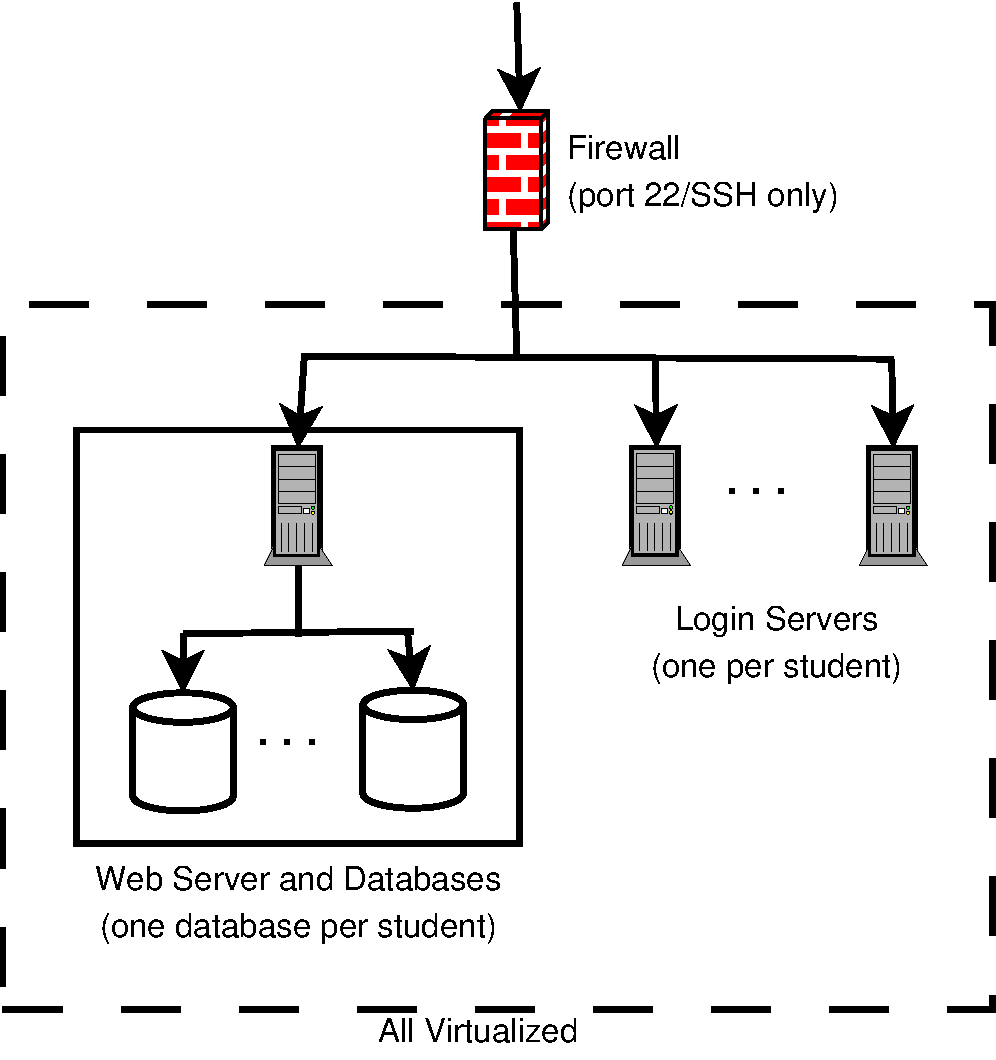
\includegraphics[width=3in]{blunderarch}
\caption{Blunderdome network architecture}
\label{fig:blunderarch}
\end{figure}

\begin{table}
\centering % TODO: fix the layout of this table.
\begin{tabular}{p{1.5in}|p{1in}|p{1in}|p{1in}}
Stage & Precondition	&	Attack	&	Postcondition \\ \hline \hline
Gain remote user access & SSH public key available (given); weak public key 
	& Break weak public key & User privileges on login server \\ \hline
Gain root access & User-level access & Execute \texttt{vmsplice} privilege escalation 
	& Root privileges on login server; access to web server credentials \\ \hline
Change grade & Address and credentials for web service & Execute SQL injection & Altered grade in database
\end{tabular}
\caption{Stages of the Blunderdome attack}
\label{table:blundertasks}
\end{table}
\TUsubsection{RFID Denial of Sleep}
The second case study used throughout this work is a denial of service attack
on the ISO 18000-7 RFID tag inventory system similar to those used by the United States
Department of Defense for shipping tracking and the Department of Energy for tracking spent
fuel containers~\cite{chen2009radiofrequency}. The attack
is similar to the ones described by Buennemeyer, \emph{et al.}~\cite{buennemeyer2006battery},
and is of a newly distinguished class of attacks sometimes termed \emph{denial
of sleep attacks}~\cite{brownfield2005wireless}~\cite{raymond2009effects}.

These ISO 18000-7 RFID tags are active and battery powered; they are used for inventory and
shipment tracking. In particular, they are used by the Department of Energy to monitor
the location and seal status of
radioactive material containers, greatly reducing workers' radiation exposure. 
The batteries on the tags should last as long as
possible in order to limit radiation exposure to maintenance workers, and
the loss of power to these devices has severe safety and security consequences.
An energy draining attack to deplete the tags' batteries could significantly
speed this loss of power.

The ISO 18000-7 tags have two modes: an active mode, and a sleep mode in which their
power consumption is significantly reduced. The active mode has a 30 second timeout,
which will cause them to sleep unless the timer is reset by the receipt of a valid
command from the reader or a wake-up signal. In sleep mode, the tags will only respond to a
wake-up command, which causes them to enter active mode.
A denial of sleep attack occurs when the tag is not permitted to enter sleep mode or is
awoken more frequently than normal.

This attack can be realized in two ways. The first is that a second, rogue 
RFID reader is placed by the attacker within range of some or all of the active tags. The
second is for the attacker to compromise an existing reader by hacking into a computer
system connected to it via a network. This presupposes that the reader is connected
to the Internet or some private network into which the attacker can intrude.

Hybrid automata serve to represent the behavior of the devices themselves quite well.
Fig.~\ref{fig:readerha} represents the reader (legitimate or rogue), which does nothing but 
transmit commands and
wake-up signals, which can come at any time with no restrictions. Under ordinary operating
conditions this might be a few times per day over the course of several years before the
batteries in the tags are drained~\cite{chen2009radiofrequency}.

Fig.~\ref{fig:tagha} depicts a model of the tags. For simplicity, they are shown as starting in
the active mode. It has two state variables: $c$, which represents the active mode timeout
clock, and $B$ represents the capacity of the battery. In active mode, the battery drains at
a rate of -50 per second, a rate chosen arbitrarily for illustrative purposes only. In sleep mode,
the battery drains at a rate of -1 per second. No restrictions are placed on the starting condition
of the battery. The two automata are composed using two shared actions: \emph{WakeUp} and \emph{Command}, which
synchronize the switches they decorate between the automata.

\begin{figure}
\centering
\begin{dot2tex}[options=-t raw --autosize]
digraph G {
    rankdir=LR;
    idle [shape=circle, texlbl= "Reading"];    
	idle -> idle [label="Command"];
	idle -> idle [label="WakeUp"];
}
\end{dot2tex}
\caption{Hybrid automaton model of the RFID reader}
\label{fig:readerha}
\end{figure}

\begin{figure}
\centering
\begin{dot2tex}[options=-t raw --autosize]
digraph G {
    rankdir=TD;
    awake [shape=circle, texlbl= \
    "$ \begin{matrix} \text{Awake} \\ \
    \dot{c}_{\lambda \mu} = -1 \wedge \dot{B}=-50 \\ \
    c>0 \wedge B>0 \end{matrix} $"];
    
    asleep [shape=circle, texlbl= \
    "$ \begin{matrix} \text{Asleep} \\ \
    \dot{c} = 1 \wedge \dot{B} = -1 \\ \
    B>0  \end{matrix}$"];
    
    dead [shape=circle, texlbl= \
    "$ \begin{matrix} \text{Dead} \\ \
    \dot{c} = 0 \wedge \dot{B} = 0 \\ \
    B=0  \end{matrix}$"];
	
	init [shape=none, label=""];
	
	init -> awake [label= " " \
    texlbl="$\begin{matrix} c=30 \
    \end{matrix}$"];
	
    awake -> awake [label= " " \
    texlbl="$\begin{matrix} \text{Command} \\ \
    c := 30 \
    \end{matrix}$"];
	
	awake -> awake [label= " " \
    texlbl="$\begin{matrix} \text{WakeUp} \\ \
    c := 30 \
    \end{matrix}$"];
	
	awake -> asleep [label= " " \
    texlbl="$\begin{matrix} \text{Timeout} \\ \
	c=0 \
    \end{matrix}$"];
	
	awake -> dead [label= " " \
    texlbl="$\begin{matrix} \text{Die} \\ \
	B=0 \
    \end{matrix}$"];
	
	asleep -> asleep [label= " " \
    texlbl="$\begin{matrix} \text{Command} \
    \end{matrix}$"];
	
	asleep -> awake [label= " " \
    texlbl="$\begin{matrix} \text{WakeUp} \\ \
    c := 30 \
    \end{matrix}$"];
    
	asleep -> dead [label= " " \
    texlbl="$\begin{matrix} \text{Die} \\ \
	B=0 \
    \end{matrix}$"];
    
	dead -> dead [label= " " \
    texlbl="$\begin{matrix} \text{Command} \
    \end{matrix}$"];
	
	dead -> dead [label= " " \
    texlbl="$\begin{matrix} \text{WakeUp} \
    \end{matrix}$"];
	
}
\end{dot2tex}
\caption{Hybrid automaton model of the case study active RFID tags}
\label{fig:tagha}
\end{figure}